\documentclass{article}
\usepackage[utf8]{inputenc}
\usepackage{enumitem,amssymb}
\usepackage{graphicx}
\usepackage{placeins}
\usepackage{subfigure}
\usepackage{tabularray}
\newlist{todolist}{itemize}{2}
\setlist[todolist]{label=$\square$}
\usepackage{pifont}
\newcommand{\cmark}{\ding{51}}%
\newcommand{\xmark}{\ding{55}}%
\newcommand{\done}{\rlap{$\square$}{\raisebox{2pt}{\large\hspace{1pt}\cmark}}%
\hspace{-2.5pt}}

\usepackage{geometry}
 \geometry{
 a4paper,
 total={170mm,257mm},
 left=20mm,
 top=20mm,
 }

\title{Paper 2 - notes}
\date{July 2024}

\begin{document}

\maketitle

\section{Introduction}
\textbf{Research Question:} How is throughput impacted when scaling is done on heterogeneous nodes?

Stuff to do:
\begin{todolist}
    \item[\done] Extend k3s deployment on heterogeneous infrastructure composed by grid5000 baremetal nodes (multi-site possible), VMs on G5k (multi-site possible), pico cluster, fit?...
    \item[\done] Implement different types of taskmanager deployment (resource limitations and configuration file) for each new type of node present in the infrastructure.
    \item[\done] Implement manual scaling technique for heterogeneous taskmanagers
    \item[\done] Preliminary test of scaling on top of heterogeneous nodes.
    \item Implement new benchmarks that are close to real world scenarios:
    \begin{itemize}
        \item yellow cab (as seen on Transscale)
        \item YSB https://github.com/yahoo/streaming-benchmarks/tree/master
        \item Theodolite use-cases?
        \item DESP-Bench https://ieeexplore.ieee.org/stamp/stamp.jsp?arnumber=9290133
    \end{itemize}

    \item Run new benchmarks with compute heterogeneity and then with netowrk heterogeneity
    \item Run full-scale real-world benchmark with multi-site deployment?
\end{todolist}


\textbf{Side Questions:}
\begin{itemize}
    \item What is the impact of the placement of the distributed storage on performance? (currently deployed on all consumer nods)
    \item Is there an additional overhead on checkpointing/savepointing when weak nodes are present?
\end{itemize}
\pagebreak

\section{Heterogeneous infrastructure}
\paragraph{Experiment setup}
\begin{figure}[h]
	\centering
	\includegraphics[width=1.0\textwidth]{images/new_cluster_deployment.png}
	\caption{New heterogeneous deployment.}
    \label{fig:heterogeneous_deployment}
\end{figure}

Figure~\ref{fig:heterogeneous_deployment} presents the new heterogeneous deployment. Two types of nodes have been added to the cluster:
\begin{itemize}
    \item VM nodes running on baremetal Grid5000 servers.
    Each VM spec can be parameterized to the desired configuration. For this reason, two types of VMs have been defined:
    \begin{itemize}
        \item \textbf{SMALL-VM}: 1 CPU cores and 2Gi of memory.
        \item \textbf{MEDIUM-VM}: 2 CPU cores and 4Gi of memory.
    \end{itemize}
    \item Raspberry Pi nodes composing a Pico cluster.
    Each node is a Raspberry Pi 4 with 4Gi of memory.
    This type of node still presents some connectivity issues due to the picocluster residing outside grid5000 network. Plumbing to fix the issue is still work in progress.
\end{itemize}

With the new infrastructure different types of TaskManagers will be deployed depending on the type node. Different resource limitations are applied on the container and multiple flink configuration files are used according to the type of node.

Baremetal nodes however can be very big. They can accommodate more than one TM at the time. For this reason and to keep their deployment proportionally big compared to the other nodes, these TM are deployed with \textbf{4 CPU cores and 16Gi of memory}.
\newpage
\section{Preliminary results: MST with heterogeneous TaskManagers running simple pipelines}

\subsection{Stateless use-case}
\begin{figure*}[h!]
    \centering
    \subfigure[BAREMETAL only]{%
        \includegraphics[width=.23\textwidth]{images/stateless/baremetal_only/experiment_plot.png}
        \label{fig:stateless_baremetal_experiment}
    }%
    \hfil
    \subfigure[BAREMETAL w MS-TM]{%
        \includegraphics[width=.23\textwidth]{images/stateless/baremetal_multitaskslot/experiment_plot.png}
        \label{fig:stateless_baremetal_multitaskslot_experiment}
    }%
    \hfil
    \subfigure[SMALL-VM only]{%
        \includegraphics[width=.23\textwidth]{images/stateless/small_vm_only/experiment_plot.png}
        \label{fig:stateless_small_vm_experiment}
    }%
    \subfigure[2 BAREMETAL + multiple SMALL-VM]{%
        \includegraphics[width=.23\textwidth]{images/stateless/baremetal_small_vm/experiment_plot.png}
        \label{fig:stateless_baremetal_small_vm_experiment}
    }%
    \\
    \subfigure[BAREMETAL only]{%
        \includegraphics[width=.23\textwidth]{images/stateless/baremetal_only/summary_plot.png}
        \label{fig:stateless_baremetal_summary}
    }%
    \hfil
    \subfigure[BAREMETAL w multi-slot TaskManager]{%
        \includegraphics[width=.23\textwidth]{images/stateless/baremetal_multitaskslot/summary_plot.png}
        \label{fig:stateless_baremetal_multitaskslot_summary}
    }%
    \hfil
    \subfigure[SMALL-VM only]{%
        \includegraphics[width=.23\textwidth]{images/stateless/small_vm_only/summary_plot.png}
        \label{fig:stateless_small_vm_summary}
    }%
    \hfil
    \subfigure[2 BAREMETAL + multiple SMALL-VM]{%
        \includegraphics[width=.23\textwidth]{images/stateless/baremetal_small_vm/summary_plot.png}
        \label{fig:stateles_baremetal_small_vm_summary}
    }%

    \caption{Stateless use-case}
    \label{fig:stateless_use_case}
\end{figure*}

\subsection{Stateful use-case}
\begin{figure*}[h!]
    \centering
    \subfigure[BAREMETAL only]{%
        \includegraphics[width=.30\textwidth]{images/stateful/baremetal_only/experiment_plot.png}
        \label{fig:stateful_baremetal_experiment}
    }%
    \hfil
    \subfigure[SMALL-VM only]{%
        \includegraphics[width=.30\textwidth]{images/stateful/small_vm_only/experiment_plot.png}
        \label{fig:stateful_small_vm_experiment}
    }%
    \hfil
    \subfigure[2 BAREMETAL + multiple SMALL-VM]{%
        \includegraphics[width=.30\textwidth]{images/stateful/baremetal_small_vm/experiment_plot.png}
        \label{fig:stateful_baremetal_small_vm_experiment}
    }%
    \\
    \subfigure[BAREMETAL only]{%
        \includegraphics[width=.30\textwidth]{images/stateful/baremetal_only/summary_plot.png}
        \label{fig:stateful_baremetal_summary}
    }%
    \hfil
    \subfigure[SMALL-VM only]{%
        \includegraphics[width=.30\textwidth]{images/stateful/small_vm_only/summary_plot.png}
        \label{fig:stateful_small_vm_summary}
    }%
    \hfil
    \subfigure[2 BAREMETAL + multiple SMALL-VM]{%
        \includegraphics[width=.30\textwidth]{images/stateful/baremetal_small_vm/summary_plot.png}
        \label{fig:stateful_baremetal_small_vm_summary}
    }%
    \caption{Stateful use-case}
    \label{fig:stateful_use_case}
\end{figure*}

\end{document}